\chapter{Analisi e progettazione}
\label{cha:analisi_progettazione}

Analizzando i vari competitor descritti nel precedente capitolo, si può notare che la maggior parte delle soluzioni presenti sul mercato sono rivolte ad una clientela qualificata. Questo probabilmente per avvicinarsi ad un utenza con più disponibilità economica.
Anche soluzioni come \textit{LongoMatch}, che offrono funzionalità più semplici, non sono progettate per un utilizzo amatoriale.

In seguito a queste analisi, ho deciso di sviluppare un'applicazione orientata ad un unico sport che fosse estremamente \textit{user-friendly}, con un'interfaccia intuitiva e con un set di funzionalità relativamente limitato. Ho deciso di focalizzarmi sulla pallavolo, uno sport che ho praticato per quasi 10 anni. Le caratteristiche di questo sport lo rendono ideale per l'analisi video, in quanto vi sono pochi giocatori e il campo ha dimensioni ridotte. Questo permette di avere una visione chiara di tutte le dinamiche di gioco, rendendole facilmente analizzabili.

La soluzione proposta è caratterizzata da un'interfaccia utente estremamente intuitiva, ideata per essere facilmente utilizzabile da utenti amatoriali. Inoltre, seguendo l'esempio della start-up \textit{BallTime}, oltre alle comuni funzionalità di analisi, ho implementato alcune funzionalità AI offrendo quindi due modalità di uso: Manuale e AI.

Le due modalità si distinguono in questo modo:
\begin{itemize}
    \item \textbf{Manuale}: Questa modalità permette di creare, importare ed esportare progetti. In particolare sono implementate le funzionalità di:
    \begin{itemize}
        \item \textit{Event Tagging}: che offre la possibilità di salvare eventi d'interesse durante l'analisi video. Sono caratterizzati dall'utilizzo di shortcut personalizzabili secondo atleta, azione e comando rapido.
        \item \textit{Drawing Tools}: attraverso cui è possibile annotare ed illustrare tattiche o azioni di gioco direttamente sul frame video.
        \item \textit{Videoclip Generator}: per generare highlights in maniera completamente automatica, partendo dagli eventi taggati. 
    \end{itemize}
    \item \textbf{AI}: Questa modalità implementa l'utilizzo di modelli di Computer Vision per l'analisi automatica dei video. In particolare sono implementate le funzionalità di:
    \begin{itemize}
        \item \textit{Ball Trajectory}: visualizzazione della traiettoria della palla durante il gioco. Disegnando una scia gialla sul video.
        \item \textit{Player Recognition}: per identificare automaticamente i giocatori in campo, assegnando ad ognuno un id e un colore di bounding box diverso.
    \end{itemize}   
\end{itemize}

\noindent I risultati dell'analisi di mercato hanno inoltre evidenziato che i prodotti si suddividono in due categorie: \textit{Desktop App} e \textit{Web App}.
Al fine di favorire il riuso su più scenari ho deciso di creare una Web App che, oltre a poter essere disponibile su un server, può essere eseguita su un computer in locale permettendo quindi scenari di servizio in cloud o di riuso su una propria macchina dedicata senza necessità di creazione di utenze

\section{Perché una Web App?}
\label{sec:web_app}

La decisione di sviluppare una Web App invece che una desktop app è basata su diversi fattori.

Una prima analisi ha delineato come l'utilizzo di siti web risulti più semplice per un target di utenza amatoriale. Questo perchè non richiede l'installazione secondo sistemi operativi specifici e può essere eseguita su un qualsiasi browser.

Questo rende l'accesso all'app semplice ed immediato, creando un'esperienza più \textit{user-friendly} con meno problematiche sul fronte della configurazione. Inoltre, offrendo potenzialmente il servizio in cloud, diventa molto più facile la gestione degli aggiornamenti in quanto saranno sempre centralizzati, rendendo l'esperienza utente più semplice e lontana da noiose installazioni manuali necessarie a garantire sempre l'ultima versione.


Un ulteriore vantaggio viene dalla funzionalità AI. Infatti, l'uso di modelli di Computer Vision richiedono risorse computazionali che non sempre sono disponibili a chiunque, sviluppando l'applicazione con interfaccia web  è possibile fare uso di tecniche di \textit{cloud computing} in cui è possibile delegare i processi computazionalmente intensi a server remoti. Questo garantisce una \textit{user-experience} il più fluida e performante possibile.

Pertanto, seguendo la volontà di creare un prodotto semplice e con basse problematiche agli utenti finali, l'approccio web è risultato quello vincente, dato che il bacino di utenza a cui si rivolge è quello di utenti amatoriali con poche disponibilità di tempo e di risorse. 

\section{Analisi dei Requisiti}
\label{sec:requisiti}

La Web App ha lo scopo di rivolgersi ad un target non professionale, quali atleti ed allenatori amatoriali. Identificandosi in questa utenza, sono state studiate le soluzioni già presenti e le funzionalità da loro proposte. In particolare, sono state prese in considerazione le feature di \textit{LongoMatch} e \textit{BallTime}, successivamente rivisitate e adattate per una \textit{user-experience} orientata a rendere il tutto più facile. 

\noindent In fase di analisi è stato fondamentale definire quelli che sono i requisiti funzionali e non funzionali del sistema.
\subsection{Requisiti Funzionali}
\label{subsec:requisiti_funzionali}

La definizione dei Requisiti Funzionali è fondamentale in fase di analisi. Ci permette infatti di identificare le funzionalità chiave che il sistema deve garantire all'utente finale. Inoltre è utile per fare un brainstorming sulla direzione che il progetto dovrà prendere.

\noindent Di seguito sono elencati i requisiti funzionali del sistema, suddivisi per categorie:

\begin{itemize}
    \item \textbf{Gestione Progetti}
    \begin{itemize}
        \item Gli utenti devono poter creare nuovi progetti, scegliendo video, giocatori e azioni.
        \item Gli utenti devono poter esportare progetti.
        \item Gli utenti devono poter importare progetti esistenti.
    \end{itemize}

    \item \textbf{Modalità e Navigazione}
    \begin{itemize}
        \item Gli utenti devono poter scegliere tra due pagine. Una gestisce l'analisi manuale e l'altra le funzionalità AI.
        \item Gli utenti devono poter navigare tra le due modalità in qualsiasi momento.
    \end{itemize}

    \item \textbf{Analisi Manuale}
    \begin{itemize}
        \item Gli utenti devono poter etichettare eventi di loro interesse durante l'analisi video.
        \item Gli eventi etichettati devono essere personalizzabili e la loro attivazione deve essere rapida.
        \item Gli eventi etichettati devono salvare dati su giocatore, azione, minutaggio e comando rapido associato.
        \item Gli eventi etichettati devono essere valutabili.
        \item Gli utenti devono poter disegnare sui frame video.
        \item Gli utenti devono poter scegliere di creare videoclip partendo degli eventi etichettati.
    \end{itemize}

    \item \textbf{Analisi AI}
    \begin{itemize}
        \item Gli utenti devono poter scegliere tra due modalità di analisi.
        \item Gli utenti devono poter visualizzare i risultati di queste analisi.
        \item Gli utenti devono poter scaricare i risultati delle analisi AI.
    \end{itemize}
\end{itemize}

\subsection{Requisiti Non Funzionali}

Lo scopo dei Requisiti Non Funzionali è quello di descrivere le caratteristiche del software che non sono definite in termini di funzionalità. Questi requisiti riguardano il funzionamento del sistema e i vincoli da rispettare per un prodotto di qualità.

\noindent Di seguito sono elencati i principali requisiti non funzionali del sistema, suddivisi in tre macroaree:

\begin{itemize}
    \item \textbf{Prestazioni}
    \begin{itemize}
        \item L'app deve garantire l'elaborazione video in tempi brevi.
        \item L'app deve essere estremamente reattiva agli input dell'utente.
    \end{itemize}

    \item \textbf{Usabilità}
    \begin{itemize}
        \item L'app deve garantire una \textit{UX} fluida e dinamica.
        \item L'app deve avere una \textit{UI} chiara ed intuitiva. 
    \end{itemize}

    \item \textbf{Compatibilità}
    \begin{itemize}
        \item L'app deve essere compatibile con i principali browser web.
        \item L'app deve adattarsi a diverse dimensioni di schermo.
    \end{itemize}
\end{itemize}

\section{Progettazione}
\label{sec:progettazione}

La progettazione della Web App ha mantenuto il focus sull'esperienza utente. Proprio per questo motivo ho creato un \textit{mockup} dell'interfaccia dell'app utilizzando Figma. 
Per avere una visione più approfondita di comportamenti e abitudini del target, ho definito due \textit{personas} e due \textit{scenari}. Durante lo sviluppo dell'applicazione ho progettato \textit{UX} e \textit{UI}, tenendo conto di questi preconcetti. 






\subsection{Personas e Scenari}
\label{subsec:personas_scenari}
\noindent Le \textit{personas} sono personaggi inventati che rappresentano possibili utenti reali. Gli \textit{scenari}, invece, descrivono dettagliatamente delle situazioni specifiche in cui l'app potrebbe essere utilizzata.
In fase di progettazione e sviluppo del prototipo Figma, definire questi concetti mi ha aiutato a capire come il target potrebbe interagire con l'applicazione.

\subsubsection{Personas}

\begin{itemize}
    \item \textbf{Marco}, 45 anni, vive a Trento ed è allenatore di una delle squadra di pallavolo Under-16 della provincia. Durante le partite è solito annotare con carta e penna le sue considerazioni rispetto alle prestazioni della squadra. Proprio a causa di questo però, gli capita spesso di perdere fasi di gioco importanti. Gli piacerebbe, quindi, poter registrare le partite, per poi fare le sue valutazioni a casa.  
     
    \item \textbf{Gaia}, 22 anni, vive a Modena ed è una giocatrice di pallavolo in una squadra universitaria. Durante le partite è solita registrarsi, chiedendo poi a suo fratello, una volta a casa, di creare highlights delle sue migliori azioni. A Gaia da fastidio non poter essere autonoma, ma proprio non riesce a prendere praticità con le app di editing video e non trova nessuna altra soluzione.
\end{itemize}

\subsubsection{Scenari}


\begin{itemize}
    \item \textbf{Scenario A}: Durante un time-out, l'allenatore raduna i giocatori attorno alla panchina. Mostra sul suo tablet il video dell'azione appena conclusa utilizzando VolleyVisionAI e con un pennino inizia a disegnare sul video, evidenziando movimenti e possibili tattiche. I giocatori hanno così istruzioni chiare su come procedere, tornando in campo più consapevoli e preparati.
    \item \textbf{Scenario B}: Prima di una gara importante, l'allenatore decide di convocare la squadra per sviluppare insieme un piano di gioco. Tramite l'utilizzo di VolleyVisionAI l'allenatore si è preparato il giorno prima dei video di alcune fasi di gioco della squadra avversaria. Successivamente ha mostrato i videoclip ai giocatori per poi interrogarli su come avrebbero reagito in determinate situazioni. Questa sessione di confronto ha permesso di migliorare l'intesa di squadra e di prepararsi per la gara.
\end{itemize}

\subsection{Struttura e Interfaccia}
\label{subsec:interfaccia}

L'utilizzo di Figma per la creazione di un prototipo della \textit{User Interface} ha permesso di capire come impostare la struttura della Web App. Il corso di \textit{EyeStudios Academy} mi ha fornito le competenze tecniche necessarie per la creazione del mockup.

VolleyVisionAI è stato ideato per avere un menu principale con due opzioni, come già descritto nell'introduzione di questo capitolo. Entrambe le funzionalità redirigono l'utente ad una nuova pagina, di seguito descritte.

La prima funzionalità, \textit{Manual}, è stata strutturata in modo da rendere chiari i tre componenti principali. Sulla destra troviamo il video player con sotto un box contenente due campi utili alla creazione degli shortcut. Sulla sinistra, invece, troviamo il contenitore di tutti gli eventi taggati fino a quel momento. Questa struttura offre una \textit{User Interface} e \textit{User Experience} semplice ed intuitiva. 

La seconda funzionalità, \textit{AI}, presenta invece un video player quasi a tutto schermo con sopra la descrizione di ciò che viene rappresentato. Questa interfaccia minimalista aiuta l'utente a concentrarsi unicamente sul risultato dell'analisi AI. 

La Web App presenta come colore predominante l'azzurro, scelto poichè trasmette tranquillità e professionalità. Inoltre le sue sfumature rendono ben leggibili i vari componenti dell'interfaccia e, allo stesso tempo, non stancano l'occhio dell'utente. In fase di progettazione, ho notato come l'azzurro fosse ideale per rappresentare il connubio tra sport e tecnologia: evoca dinamismo ed energia, tipici dello sport, e trasmette al contempo freschezza e innovazione, caratteristiche della tecnologia. Così, l'azzurro bilancia intensità e modernità, rendendo l'interfaccia armoniosa ed efficace.

\begin{figure}[htb]
    \centering 
    \begin{subfigure}{0.48\textwidth}
        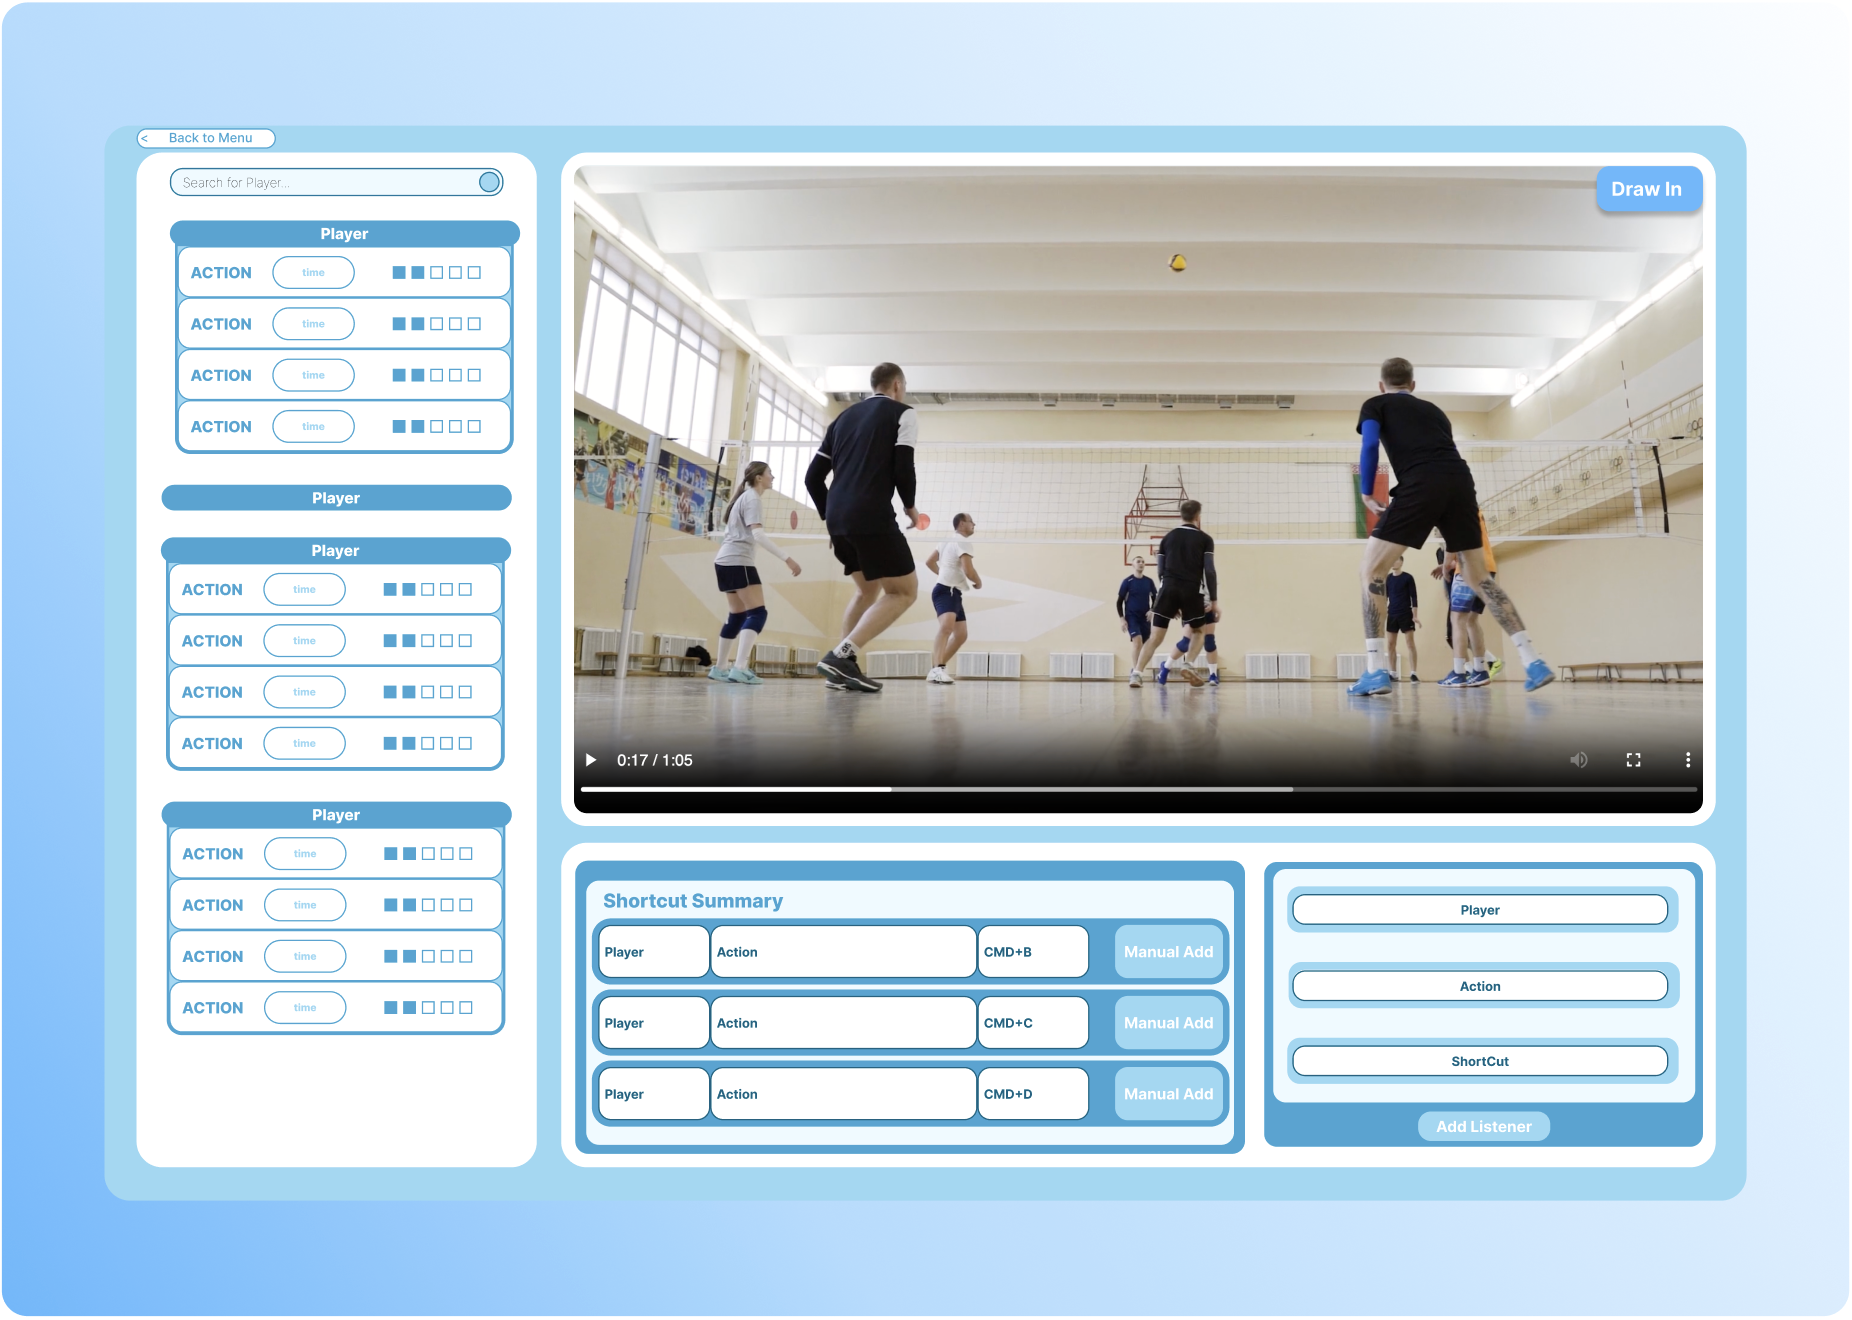
\includegraphics[width=\linewidth]{img/figma_manual.png}
        \caption{Mockup Analisi Manuale}
        \label{fig:mokup_manual}
    \end{subfigure}\hspace{0.04\textwidth}% Aggiunge uno spazio tra le due immagini
    \begin{subfigure}{0.48\textwidth}
        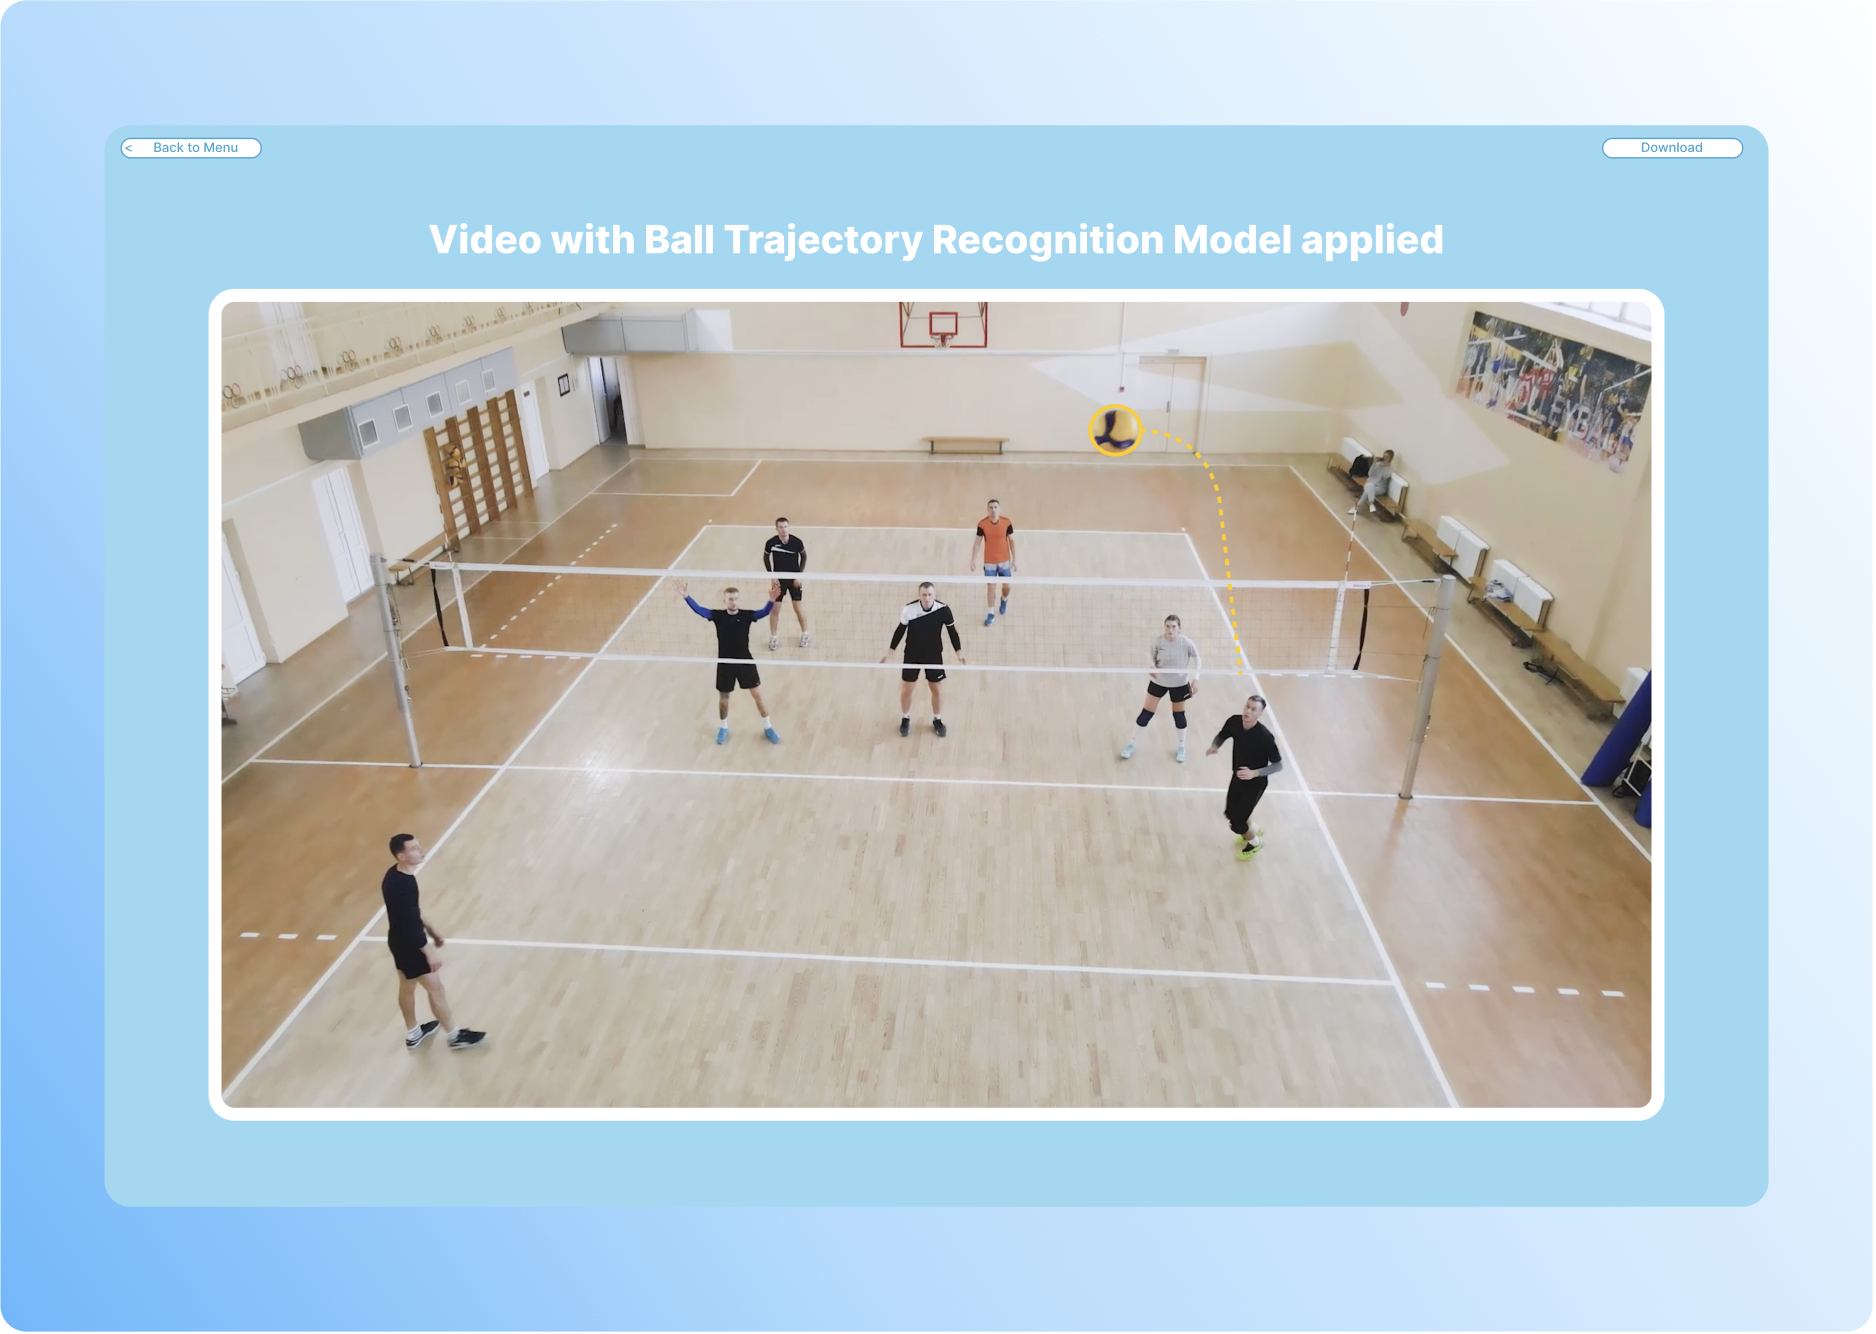
\includegraphics[width=\linewidth]{img/figma_ai.png}
        \caption{Mockup Analisi AI}
        \label{fig:mokup_ai}
    \end{subfigure}
    \caption{Figma Mockup}
    \label{fig:bot_competitor}
\end{figure}

\subsection{Server}
\label{sec:subserver}


Per garantire una manipolazione efficiente dei video e l'implementazione dei modelli di \textit{Computer Vision}, è stato necessario sviluppare un server back-end robusto e affidabile. Questo server svolge un ruolo cruciale nella gestione delle operazioni computazionalmente intensive, liberando i dispositivi degli utenti dal carico di elaborazione e assicurando un'esperienza d'uso fluida e performante.
Il Server è connesso direttamente al front-end della Web App tramite API , consentendo una comunicazione rapida e sicura tra l'interfaccia utente e il back-end. Questo permette di ricevere richieste, elaborare i dati dei video tramite i modelli di \textit{Computer Vision} e restituire i risultati all'utente in tempo reale.
